\def\SECTION{2.3 Postulates \& Diagrams}
\documentclass[aspectratio=169,14pt]{beamer}
\usepackage[T1]{fontenc}
\usepackage{mathpazo}
\usepackage{amsmath,amssymb}
\usepackage{tikz}
\usetikzlibrary{arrows.meta,calc,decorations.pathreplacing}
\definecolor{fblue}{HTML}{1F4E79}
\definecolor{fteal}{HTML}{0F7C7C}
\definecolor{fgold}{HTML}{C9962B}
\definecolor{fred}{HTML}{B3261E}
\definecolor{fink}{HTML}{16233B}
\definecolor{fsoft}{HTML}{EEF3F8}
\definecolor{fgoldsoft}{HTML}{FBF1DC}
\setbeamertemplate{navigation symbols}{}
\setbeamercolor{normal text}{fg=fink}
\setbeamercolor{frametitle}{fg=fblue}
\setbeamerfont{frametitle}{series=\bfseries,size=\Large}
\setbeamercolor{structure}{fg=fteal}
\setbeamertemplate{itemize item}{\color{fteal}$\blacktriangleright$}
\setbeamertemplate{frametitle}{\vspace{6pt}\insertframetitle\par\vspace{-2pt}{\color{fgold}\rule{2.2cm}{2pt}}}
\setbeamertemplate{footline}{\hspace{0.6cm}{\color{fblue}\scriptsize\bfseries Fang\textcolor{fteal}{Math}}\hfill{\scriptsize\color{gray}\SECTION\quad\insertframenumber}\hspace{0.6cm}\vspace{6pt}}
\newcommand{\key}[1]{{\color{fteal}\textbf{#1}}}
\newcommand{\ans}[1]{\colorbox{fgoldsoft}{\color{fink}\ensuremath{#1}}}
\newcommand{\warn}[1]{\begin{beamercolorbox}[sep=8pt,rounded=true]{warnbox}{\color{fred}\textbf{Watch out!}}\enskip #1\end{beamercolorbox}}
\setbeamercolor{warnbox}{bg=fred!8,fg=fink}
\setbeamercolor{turnbox}{bg=fgoldsoft,fg=fink}
\setbeamercolor{defbox}{bg=fsoft,fg=fink}
\newcommand{\defn}[1]{\begin{beamercolorbox}[sep=8pt,rounded=true]{defbox}#1\end{beamercolorbox}}
\newenvironment{yourturn}{\begin{beamercolorbox}[sep=10pt,rounded=true]{turnbox}{\color{fgold}\Large\bfseries Your turn!}\quad{\small Pause the video and try it.}\par\medskip}{\end{beamercolorbox}}
\newcommand{\titleframe}[3]{%
\begin{frame}[plain]
\begin{tikzpicture}[remember picture,overlay]
\fill[fblue] (current page.north west) rectangle ([yshift=-0.9cm]current page.north east);
\node[anchor=west,text=white,font=\bfseries] at ([xshift=0.6cm,yshift=-0.45cm]current page.north west) {Fang\textcolor{fgold}{Math}};
\node[anchor=east,text=white,font=\small] at ([xshift=-0.6cm,yshift=-0.45cm]current page.north east) {Geometry $\cdot$ Chapter \CHNO};
\end{tikzpicture}
\vfill
{\color{fteal}\large\bfseries #1}\par\medskip
{\color{fblue}\fontsize{30}{34}\selectfont\bfseries #2}\par\medskip
{\color{fgold}\rule{3cm}{3pt}}\par\bigskip
{\large #3}
\vfill
{\small\color{gray} fangmath.com $\cdot$ YouTube @fangmathcom}
\end{frame}}
\newcommand{\closeframe}[1]{%
\begin{frame}{Remember}
#1
\vfill
\begin{center}{\color{fblue}\large\bfseries Now practice at your level:}\par\smallskip
{\Large\color{fteal}\bfseries fangmath.com} \enskip{\color{gray}$\to$ Geometry $\to$ Chapter \CHNO}\end{center}
\end{frame}}

\usepackage{pgfplots}\pgfplotsset{compat=1.17}
\newcommand{\grid}[4]{\draw[step=1,gray!25] (#1,#2) grid (#3,#4);\draw[-{Stealth},gray] (#1,0)--(#3+0.3,0) node[right]{\small$x$};\draw[-{Stealth},gray] (0,#2)--(0,#4+0.3) node[above]{\small$y$};}
\def\CHNO{2}
\usetikzlibrary{angles,quotes}
\begin{document}
\titleframe{Lesson 2.3}{Postulates \& Diagrams}{Rules we accept --- and what a picture really tells you}
\begin{frame}{What is a postulate?}
\onslide<1->{\defn{A \key{postulate} is a rule we accept as true \textbf{without proof}. Everything else in geometry is built on postulates.}}\par\medskip
\end{frame}
\begin{frame}{Point, line and plane postulates}
\onslide<1->{\tikz[baseline=-3pt]{\draw[thick] (0,0)--(1.4,0); \fill (0.2,0) circle(2pt) (1.2,0) circle(2pt);} \ Through any \textbf{two points} there is exactly \key{one line}.}\par\medskip
\onslide<2->{\tikz[baseline=-3pt]{\fill[fteal!15] (0,-0.2)--(1.2,-0.2)--(1.5,0.3)--(0.3,0.3)--cycle; \fill (0.3,-0.05) circle(2pt) (1.1,0) circle(2pt) (0.7,0.2) circle(2pt);} \ Through any \textbf{three noncollinear points} there is exactly \key{one plane}.}\par\medskip
\onslide<3->{\tikz[baseline=-3pt]{\draw[thick] (0,-0.25)--(1,0.25) (0,0.25)--(1,-0.25); \fill[fred] (0.5,0) circle(2pt);} \ Two lines meet in exactly \key{one point}.}\par\medskip
\onslide<4->{\tikz[baseline=-3pt]{\fill[fteal!15] (0,-0.25)--(1.2,-0.25)--(1.4,0.15)--(0.2,0.15)--cycle; \draw[fred,thick] (0.7,-0.25)--(0.7,0.35);} \ Two planes meet in exactly \key{one line}.}\par\medskip
\end{frame}
\begin{frame}{Reading a diagram}
\begin{columns}[c]\begin{column}{0.44\textwidth}\centering 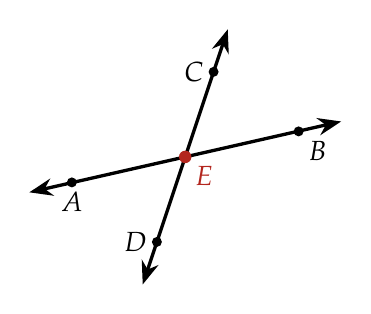
\begin{tikzpicture}[scale=0.9]\draw[very thick,{Stealth}-{Stealth}] (-2.2,-0.5)--(2.2,0.5); \draw[very thick,{Stealth}-{Stealth}] (-0.6,-1.8)--(0.6,1.8); \fill (-1.6,-0.36) circle(2pt) node[below]{$A$} (1.6,0.36) circle(2pt) node[below right]{$B$} (-0.4,-1.2) circle(2pt) node[left]{$D$} (0.4,1.2) circle(2pt) node[left]{$C$}; \fill[fred] (0,0) circle(2.5pt) node[below right]{$E$};\end{tikzpicture}\end{column}\begin{column}{0.54\textwidth}\onslide<1->{You \key{can} assume: $A$, $E$, $B$ are collinear \checkmark}\par\medskip
\onslide<2->{You \key{can} assume: the two lines meet at $E$ \checkmark}\par\medskip
\onslide<3->{You \textbf{cannot} assume: $\angle AEC = 90^\circ$ \ {\color{fred}$\times$} \ (no right-angle mark)}\par\medskip
\onslide<4->{You \textbf{cannot} assume: $AE = EB$ \ {\color{fred}$\times$} \ (no tick marks)}\par\medskip\end{column}\end{columns}
\end{frame}
\begin{frame}{Marks tell you sizes}
\onslide<1->{\tikz[baseline=0]{\draw[thick] (0,0)--(1,0) (0,0)--(0,1); \draw (0.2,0)--(0.2,0.2)--(0,0.2);} \ right angle \qquad \tikz[baseline=0]{\draw[thick] (0,0.2)--(1.2,0.2); \draw (0.3,0.1)--(0.3,0.3) (0.9,0.1)--(0.9,0.3);} \ equal lengths \qquad \tikz[baseline=0]{\draw[thick,-{Stealth}] (0,0.4)--(1.2,0.4); \draw[thick,-{Stealth}] (0,0)--(1.2,0); \draw[thick] (0.5,0.3)--(0.6,0.4)--(0.5,0.5) (0.5,-0.1)--(0.6,0)--(0.5,0.1);} \ parallel}\par\medskip
\end{frame}
\begin{frame}{Watch out}
\onslide<1->{\warn{``It looks like it'' is \textbf{not} a reason. Only what is \textbf{drawn} (position) or \textbf{marked} (size) counts.}}\par\medskip
\end{frame}
\begin{frame}{}
\begin{columns}[c]\begin{column}{0.6\textwidth}\begin{yourturn}Which can you assume? \\ (a) $A$, $P$, $B$ are collinear \quad (b) $PA = PB$ \quad (c) the lines are perpendicular\end{yourturn}\par\medskip
\onslide<2->{(a) \ans{\text{yes}} --- drawn on one line. \quad (b) \ans{\text{yes}} --- tick marks. \quad (c) \ans{\text{no}} --- no right-angle mark.}\par\medskip\end{column}\begin{column}{0.38\textwidth}\centering 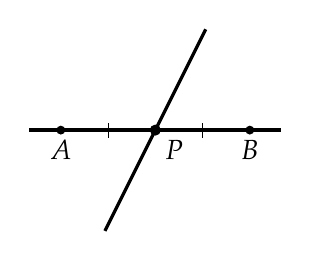
\begin{tikzpicture}[scale=0.8]\draw[very thick] (-2,0)--(2,0); \draw[very thick] (-0.8,-1.6)--(0.8,1.6); \fill (-1.5,0) circle(2pt) node[below]{$A$} (1.5,0) circle(2pt) node[below]{$B$} (0,0) circle(2.5pt) node[below right]{$P$}; \draw (-0.75,-0.12)--(-0.75,0.12) (0.75,-0.12)--(0.75,0.12);\end{tikzpicture}\end{column}\end{columns}
\end{frame}
\closeframe{\begin{itemize}\setlength\itemsep{8pt}
\item Two points $\to$ one line; three noncollinear points $\to$ one plane.
\item Two lines meet in a point; two planes meet in a line.
\item Assume what is \key{drawn}, not sizes --- unless they are \key{marked}.
\end{itemize}}
\end{document}
